\documentclass[12pt,a4paper]{article}
\usepackage[T1]{fontenc}
\usepackage[utf8]{inputenc}
\usepackage[margin=25mm]{geometry}
\usepackage{graphicx,booktabs,amsmath,tabularx,array,microtype,xcolor}
\usepackage{tikz}
\usetikzlibrary{arrows.meta,positioning}
\usepackage[labelfont=bf,font=small]{caption}
\usepackage{xurl}
\usepackage[hidelinks]{hyperref}
\usepackage{float,placeins,fancyhdr}
\setlength{\parindent}{0pt}
\setlength{\parskip}{5pt plus 1pt}
\fancyhf{}\fancyfoot[C]{\thepage}\renewcommand{\headrulewidth}{0pt}\pagestyle{fancy}
\newcommand{\resultsroot}{../output/final-results/}
% All imported graphics resolve beneath resultsroot. Missing exports stay visible.
\newcommand{\resultimage}[2]{\IfFileExists{\resultsroot#2}{\includegraphics[width=#1]{\resultsroot#2}}{\fbox{\begin{minipage}[c][26mm][c]{\dimexpr#1-2\fboxsep-2\fboxrule\relax}\centering\small\textbf{Missing code export}\\[3pt]\scriptsize\path{#2}\end{minipage}}}}
\newcommand{\panel}[3]{\begin{minipage}[t]{#1}\centering\resultimage{\linewidth}{#2}\\[2pt]{\scriptsize #3}\end{minipage}}
\newcommand{\validation}{\par\textbf{Validation and decision.}\ }
\begin{document}
\begin{center}
{\Large\bfseries Pool-ball localisation and recognition}\\[4pt]
Computer Vision (CSU44053)\\
Manon Yiqin Galian Ng (23375206)
\end{center}

\section{Introduction}
The objective of this project was to locate pool balls in photographs of a table and identify each ball by 
type and number. The task was divided into detecting candidate balls and recognising their identities. 

The development process was iterative. 
I began with simple threshold-based methods, inspected intermediate images and quantitative errors, 
and introduced more advanced methods to try to solve the issues where the earlier solutions were unreliable. 
The training AllBalls.jpeg image supplied Hough parameter selection and reference colour modelling. 
Tables1--6 were used repeatedly to validate and refine the solution. 

\section{Detailed Design and Evaluation Overview}
\subsection{Final Pipeline overview}

\begin{figure}[H]
\centering
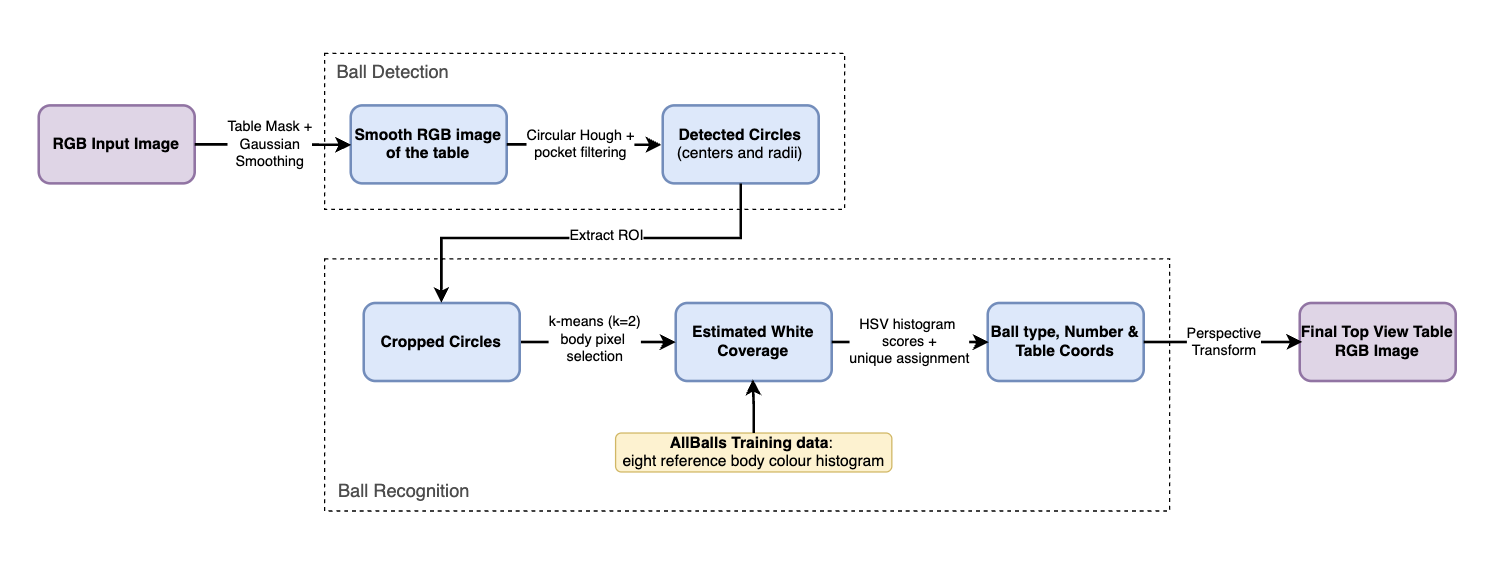
\includegraphics[width=\linewidth]{assets/pipeline.png}
\caption{Overview of the pool-ball localisation and recognition pipeline.}
\label{fig:pipeline}
\end{figure}

\subsection{Evaluation Methodalogy}
Tables1--6 contain 90 annotated balls. Predictions are matched one-to-one to ground-truth centres within 15 units in the rectified table coordinate system. Matching prioritises the number of valid pairs and uses proximity to resolve alternatives; it does not necessarily minimise total distance globally. A matched detection is a true positive (TP); unmatched predictions are false positives (FP), and unmatched annotations are false negatives (FN).
\[
P=\frac{TP}{TP+FP},\qquad R=\frac{TP}{TP+FN},\qquad F_1=\frac{2PR}{P+R}.
\]
Mean localisation error is the mean Euclidean distance of matched pairs. Recognition experiments distinguish \emph{type accuracy} (cue/solid/striped) from \emph{identity accuracy} (cue or exact number). Identity accuracy uses matched detections as its denominator; end-to-end correct-identity recall uses all 90 annotations, so missed balls also count against it. An Unknown prediction on a genuine ball is an identity error. End-to-end recall does not directly penalise extra detections, which remain visible in precision and FP counts.

\subsection{Ball Detection}
\subsubsection{Table masking and smoothing}
The first step restricts processing to the table. The supplied corners are top-left 
$(337,35)$, top-right $(1570,21)$, bottom-right $(1888,451)$ and bottom-left 
$(38,472)$ in original-image coordinates. I use them to create a quadrilateral mask and 
set the background outside the table surface to black. The masked image was then 
converted to greyscale and smoothed with a $5\times5$ Gaussian filter ($\sigma=1.5$). 
This reduces small intensity variations while preserving approximate ball boundaries.

\begin{figure}[H]\centering
\panel{.48\linewidth}{mainDetectionResults/AllBalls/masked.png}{Table mask applied}\hfill
\panel{.48\linewidth}{mainDetectionResults/AllBalls/blurred.png}{Greyscale and Gaussian smoothing}
\caption{Preprocessing exports on AllBalls.}
\end{figure}

\subsubsection{Circular Hough transform and parameter search}
I used OpenCV's gradient-based Circular Hough Transform to find candidate ball
centres and radii. I initially adjusted the parameters manually on
AllBalls.jpeg and inspected the detected circles. This was slow and
made it difficult to compare missed balls with false detections, so I switched
to a grid search.

All configurations used the same annotations, coordinate transform and 15-unit 
matching tolerance. They were ranked first by matched balls, then by false positives 
and mean centre error. Recall was prioritised because recognition cannot recover a 
ball for which no candidate exists. The selected parameters were accumulator 
resolution ratio 1.5, minimum centre separation 18 pixels, edge threshold 75 and 
circle threshold 35.

The search evaluated 480 combinations of accumulator resolution, minimum centre 
separation, edge threshold, and circle accumulator threshold, while keeping the 
radius range fixed at 15–30 pixels.
For each combination, I transformed the detected centres
into table coordinates and compared them with the annotations, using a
15-unit matching tolerance. I ranked the configurations by the number of
correctly detected balls, then by false positives, and finally by mean centre
error. I prioritised recall because any ball missed at this stage could not
be recognised later. The selected settings were an accumulator resolution
ratio of 1.5, minimum centre separation of 18 pixels, edge threshold of 75
and circle threshold of 35.

\validation The saved grid-search row gave 16 TP, 1 FP and 0 FN on AllBalls: 
100\% recall, 94.12\% precision, 96.97\% F1 and mean error 2.76 table units.  
The same settings were then used on all six development images. 

\subsubsection{Pocket filtering}
Pockets resemble dark circular objects. I transform candidate centres to table 
coordinates and reject those within 25 units of six approximate pocket centres. 
This geometry-based filter is retained in the selected pipeline, 
although it could reject a genuine ball sufficiently close to a pocket.

\validation The final detection results on AllBalls are 16 TP, 1 FP and 0 FN before filtering, and 16 TP, 0 FP and 0 FN after filtering.
For the remaining images we have TODO.

\begin{figure}[H]\centering
\panel{.48\linewidth}{mainDetectionResults/AllBalls/raw_circles.png}{Before pocket filtering}\hfill
\panel{.48\linewidth}{mainDetectionResults/AllBalls/filtered_circles.png}{After pocket filtering}
\caption{Detection results on AllBalls.}
\end{figure}

\subsubsection{Additional Detection Experiments: TODO}
Touching balls have interrupted outlines, so I investigated segmentation-assisted recovery. The reconstructed watershed experiment builds foreground regions and distance-transform/watershed proposals around the baseline detections. Area, shape, support, duplicate and pocket checks decide whether to accept additional circles. The reconstructed guided-Hough experiment instead searches foreground regions with more permissive local circle settings.

\begin{figure}[H]\centering
\panel{.32\linewidth}{ExperimentWatershedResults/Table1/foreground.png}{Foreground}\hfill
\panel{.32\linewidth}{ExperimentWatershedResults/Table1/distance.png}{Distance transform}\hfill
\panel{.32\linewidth}{ExperimentWatershedResults/Table1/basins.png}{Watershed basins}
\caption{Reconstructed watershed diagnostics on the crowded Table1 scene. Segmentation appearance alone does not establish an extra true detection.}
\end{figure}
\begin{table}[H]\centering\small
\caption{Detection comparison on the same six development images. F1 is calculated from pooled counts, not averaged image percentages.}
\begin{tabular}{lrrrr}\toprule
Configuration & TP & FP & FN & F1 (\%)\\\midrule
Selected global Hough + filtering &86&2&4&96.63\\
Reconstructed watershed &86&2&4&96.63\\
Reconstructed guided Hough &87&17&3&89.69\\\bottomrule
\end{tabular}
\end{table}
\validation Watershed makes no accepted change to detections. Guided Hough recovers one additional matched ball but adds 15 false detections across the six images. On Table4, its local success is 14 TP/0 FP/1 FN becoming 15 TP/2 FP/0 FN. The pooled F1 reduction supports retaining the simpler global detector. These are the reconstructed variants saved with the final results; the original guided detector used a different replacement procedure and must not be assigned these numbers.
\begin{figure}[H]\centering
\panel{.48\linewidth}{mainDetectionResults/Table4/filtered_circles.png}{Baseline: 14 TP, 0 FP, 1 FN}\hfill
\panel{.48\linewidth}{ExperimentGuidedHoughResults/Table4/circles.png}{Guided Hough: 15 TP, 2 FP, 0 FN}
\caption{A recovered ball with an accompanying false-detection cost on Table4.}
\end{figure}

\subsubsection{Ball extraction}
I cropped each detected ball from the original colour image and applied a
circular mask to prepare it for recognition. This also made it easier to
inspect the processing steps for each ball individually.

\subsection{Ball Recognition -- Type}
\subsubsection{HLS thresholding}
My first approach classified pixels by HLS lightness and saturation into white, 
dark and coloured categories. Their fractions within the circular mask supplied hard 
cue/solid/stripe rules. Fixed thresholds are easy to interpret but sensitive to highlights, 
shadows and crop boundaries.

This HLS baseline only correctly classifies 43/86 matched development detections by type (50.00\%).
TODO: add performance on AllBalls. 
A resonable next step was to use k-means clustering, which groups pixels by their colour 
values rather than relying on fixed thresholds to separate them. 

TODO: Add the correct images
\begin{figure}[H]\centering
\panel{.48\linewidth}{ExperimentManualHLSResults/AllBalls/predicted_types.png}{Requested training-image HLS result}\hfill
\panel{.48\linewidth}{ExperimentManualHLSResults/Table1/predicted_types.png}{Available Table1 HLS predictions}
\caption{Manual-threshold type predictions.}
\end{figure}

\subsubsection{K-means ball-type estimation}
The next approach involved clustering the ball pixels in BGR colour space, starting with
two clusters. The idea was that the white and coloured regions of a striped
ball would often form separate groups. Each cluster's mean was converted from BGR
colour to HSV and labelled it as light, dark or coloured, then used the
cluster sizes to estimate how much of the ball belonged to each category.
A cluster was considered light when $V \ge 170$ and $S \le 165$.
A non-light cluster with $V \le 90$ was considered dark. These were
manually selected thresholds.

Initially, simple rules were used to classify the ball type: at least 85\%
light coverage indicated a cue-ball candidate, while at least 70\%
non-light coverage indicated a solid. The remaining cases with a mix of
light and non-light pixels were labelled striped.

\validation This approach correctly classified all 16 balls in \texttt{AllBalls.jpeg}
and 76 of the 86 matched detections across the six development images.
These results encouraged me to keep $K=2$. I also considered larger values
of $K$ but there performance was worse than the selected $K=2$ given the current
thresholds and rules.

\begin{table}[H]\centering\small
\caption{Reconstructed type comparisons on the same 86 matched detections. Colour identities are not evaluated by these rows.}
\begin{tabular}{lrr}\toprule
Method & Correct types & Accuracy (\%)\\\midrule
Manual HLS &43&50.00\\
K=2 &76&88.37\\
K=3, K=4 or K=5 &73&84.88\\
K=6 &74&86.05\\
\end{tabular}
\end{table}

TODO: Add the correct images
\begin{figure}[H]\centering
\panel{.48\linewidth}{ExperimentKMeansK2Results/AllBalls/predicted_types.png}{Requested AllBalls initial K=2 types}\hfill
\panel{.48\linewidth}{ExperimentKMeansK2Results/Table2/predicted_types.png}{Available Table2 initial K=2 types}
\caption{Training and development views of the initial type estimator. The final AllBalls identity overlay would include later corrections and cannot replace the missing initial-type export.}
\end{figure}

\subsubsection{Connected-component analysis}
K-means estimates how much of each colour is present, but does not describe
where those colours appear on the ball. I therefore tested connected-component
analysis (CCA) to examine the arrangement of light and non-light regions.
I looked at the number of connected regions, the proportion covered by the
largest regions, and the amount of light coverage near the ball's boundary.
My idea was that a stripe's larger white regions could help distinguish it
from the small white number patch on a solid ball. However, ball orientation,
highlights and shadows could also affect how these regions connected.

TODO: add the correct images (needs to show the short commings)
\begin{figure}[H]\centering
\panel{.20\linewidth}{ExperimentCCAResults/Table1/ball_7_light.png}{Candidate 7 light mask}\hfill
\panel{.20\linewidth}{ExperimentCCAResults/Table1/ball_9_light.png}{Candidate 9 light mask}\hfill
\panel{.55\linewidth}{ExperimentCCAResults/Table1/predicted_types.png}{CCA type predictions on Table1}
\caption{Spatial evidence supplied to the reconstructed CCA rule. Light masks show the regions being analysed, rather than ground-truth stripes.}
\end{figure}
\validation When tested on the same 86 matched detections, the reconstructed
CCA approach reduced the number of correct type classifications from 76
to 73. Since CCA did not improve either result, I left it out of the selected pipeline.

\subsection{Ball Recognition -- Colour}
\subsubsection{K means colour classification}
Initially, I used the representative colour of a K-means cluster and HSV
hue thresholds to classify balls as yellow, blue, red, purple, orange,
green or maroon. I used a separate low-value threshold for black, since
hue alone was not useful for identifying it. These rules were easy to
interpret, but similar colours were difficult to separate reliably.
Reflections and shading could also shift the cluster's mean colour across
a threshold. This led me to try colour histograms, which describe the
distribution of colours rather than relying on a single mean.

\validation The reconstructed hue-based classifier correctly identified
68 of the 86 matched detections (79.07\%).

TODO: Add images for short comings
\begin{figure}[H]\centering
\panel{.48\linewidth}{ExperimentKMeansHueResults/Table1/table_numbered.png}{Independent centroid/hue classifier}\hfill
\panel{.48\linewidth}{mainFinalResults/Table1/table_numbered.png}{Complete selected recogniser}
\caption{Table1 identity outputs with the same detection geometry. Several recognition stages differ between panels.}
\end{figure}

\subsubsection{Reference HSV histograms}
I built eight reference body-colour histograms from labelled examples in
AllBalls.jpeg, using a shared model for solid and striped balls
of the same colour. The cue ball was excluded. Before calculating each
histogram, I slightly shrank the circular mask using a $3\times3$ elliptical
erosion kernel and removed bright, low-saturation pixels. This helped
reduce the influence of the crop boundary, white patches and reflections,
so the histogram focused on the ball's body colour. If fewer than 12 usable
pixels remained, I did not use the crop as colour evidence for a numbered ball.

Each histogram used 18 hue bins, eight saturation bins and eight value
bins, giving $18\times8\times8=1152$ bins in total. In OpenCV's HSV
representation, hue ranges from $[0,180)$, while saturation and value
range from $[0,256)$. Each hue bin therefore covers 10 OpenCV hue units,
and each saturation and value bin covers 32 levels. This gives a finer
division of hue to help distinguish body colours, while keeping saturation
and value more broadly grouped to allow for differences in lighting.
The bin counts provide a compromise between preserving colour detail
and avoiding a histogram that is too sensitive to small pixel changes.

For nearly grey pixels, defined here as a difference of less than 15
between the largest and smallest BGR values, I set hue to zero because
hue is unreliable when there is little colour variation. I then smoothed
each histogram axis using a $[1,2,1]/4$ filter. This gives neighbouring
bins some shared weight, reducing the effect of colours falling just
either side of a bin boundary. Hue wraps around at its endpoints, while
saturation and value use repeated endpoint values. Finally, I normalised
each histogram to sum to one and gave the solid and striped reference
examples equal weight.

For each candidate ball, I calculated the same histogram and compared it
with all eight references. I converted the Bhattacharyya distance into
a similarity score using:
\[
s(p,q)=1-\sqrt{1-\sum_b\sqrt{p_bq_b}},
\]
where $p$ and $q$ are normalised histograms and $b$ indexes the bins.
A higher score indicates a closer match. This gave eight possible
body-colour scores for identity assignment, rather than a single fixed
colour label. I also used backprojection images to inspect which pixels
matched each reference distribution. The scores used for recognition
came from the direct histogram comparisons.

\begin{figure}[H]\centering
\panel{.23\linewidth}{mainTypeRecognitionResults/Table3/ball_8_kmeans.png}{K=2 segmentation}\hfill
\panel{.23\linewidth}{mainColourRecognitionResults/Table3/ball_8_body.png}{Body-colour pixels}\hfill
\panel{.23\linewidth}{ExperimentHistogramBackprojectionResults/Table3/ball_8_bestColour.png}{Best-colour backprojection}\hfill
\panel{.23\linewidth}{mainColourRecognitionResults/Table3/ball_8_histogram.png}{Requested histogram plot}
\caption{Available colour diagnostics for Table3 candidate 8. The backprojection is from the reconstructed diagnostic run; it is not a final identity probability or a controlled before/after panel. No histogram plot is currently exported.}
\end{figure}

\validation In the original controlled colour experiment with fixed K=2 types and detections, 
replacing the colour rules with HSV histograms improves identities from 68/86 to 72/86, 
with four fixes and no losses against that control. 

\subsubsection{Continuous ball-type compatibility}
Next I wanted to address the pool ball property that all ball are unique.
With fixed thresholds, two balls with almost the same light coverage could
be assigned different types simply because they fall on opposite sides of
a boundary. I therefore replaced the hard rules with scores that describe
how well each ball fits each type. I kept the same expected light-fraction
ranges: $[0,0.30]$ for solids, $[0.30,0.85]$ for stripes and $[0.85,1]$
for the cue ball.

For a measured light fraction $w$ and the expected interval $I_t$ for
type $t$, I calculated:
\[
g_t(w)=\exp\left(-\frac{d(w,I_t)^2}{2(0.10)^2}\right),
\]
where $d$ is zero when $w$ falls inside the interval, and otherwise is
the distance to the nearest endpoint. A ball receives a score of one
within the expected range, with the score gradually decreasing outside
it. The width parameter, 0.10, controls how quickly this decrease happens.
These scores express compatibility.

For each numbered identity, I multiplied the colour similarity by the
score for its type. For the cue ball, I used $w g_{\mathrm{cue}}(w)$,
so greater light coverage also increased its score.

Each numbered ball can appear at most once, but classifying candidates
independently can produce duplicate identities. To account for this,
I arranged the candidate-to-identity scores in a matrix and used the
Hungarian algorithm to maximise the total score while assigning each
identity at most once. Extra dummy columns allowed multiple candidates
to be labelled \texttt{Unknown}. 

\validation Using the same 86 matched detections, replacing hard
classification with independent soft scores increased correct identities
from 72 to 73. Adding unique assignment then increased this to 75.
The improvement therefore came from both changes. 

TODO: Add images 
\begin{figure}[H]\centering
\panel{.48\linewidth}{ExperimentSoftTypeResults/Table3/hard_types.png}{Requested hard-type identity control}\hfill
\panel{.48\linewidth}{ExperimentSoftTypeResults/Table3/soft_types.png}{Requested independent soft-score output}
\caption{Required controlled visual exports for soft scoring. Final selected predictions cannot substitute for the missing intermediate configurations.}
\end{figure}

\subsubsection{Cue-ball ambiguity and selective crop expansion}
When inspecting the results, I noticed that the Hough transform sometimes
detected a white number patch or another bright region inside a ball
instead of its full outline. This could cause more than one candidate
to be initially classified as white. I made two changes to address this.

First, I expanded the recognition crop radius of initially white candidates
by one pixel, then recalculated their type and colour scores. This left
the stored detection centre and original Hough radius unchanged. Second,
when several candidates were initially classified as white, I reserved
the cue identity for the one with the largest original Hough radius.
For example, on \texttt{Table1}, the actual cue ball had a detected radius
of 24.15 pixels, compared with 17.55 pixels for the competing white patch.

\validation Expanding these crops increased correct identities from
75/86 to 79/86, with no previously correct identities becoming incorrect.
The cue selection rule increased this further to 80/86 and improved cue
recognition from 5/6 to 6/6. The original rule that adjusted radius by
image row produced the same cue choices and overall result, so I kept
the simpler largest-radius rule. A separately reconstructed expected-radius
rule achieved 75/86, but used a different heuristic and did not reproduce
the original row-adjusted method.

\begin{figure}[H]\centering
\panel{.32\linewidth}{ExperimentCuePaddingResults/Table1/unpadded_numbered.png}{Requested: assignment before padding}\hfill
\panel{.32\linewidth}{ExperimentCuePaddingResults/Table1/padded_numbered.png}{Requested: +1 padding, no cue reservation}\hfill
\panel{.32\linewidth}{mainFinalResults/Table1/table_numbered.png}{Available: padding + raw-radius reservation}
\caption{Requested cue-correction comparison on Table1. Only the complete selected run is currently available in final-results.}
\end{figure}
\begin{figure}[H]\centering
\panel{.23\linewidth}{mainBallExtractionResults/Table1/ball_6_original.png}{Genuine cue, original crop}\hfill
\panel{.23\linewidth}{mainBallExtractionResults/Table1/ball_7_original.png}{Competing white patch}\hfill
\panel{.23\linewidth}{mainColourRecognitionResults/Table1/ball_6_body.png}{Cue body evidence after padding}\hfill
\panel{.23\linewidth}{mainColourRecognitionResults/Table1/ball_7_body.png}{Patch body evidence after padding}
\caption{Candidate-level evidence for cue ambiguity. Original-colour crop exports are needed to interpret the available body masks directly.}
\end{figure}

\subsection{Results transformation and Visualisation}
The four supplied corners define a homography to $(0,0)$, $(1433,0)$, $(1433,682)$ and $(0,682)$ in a $1434\times683$ rectangle. It has the form $\lambda(x_t,y_t,1)^T=H(x,y,1)^T$. At the supplied table scale, a coordinate unit is approximately one millimetre. Hough detection and colour measurements remain in the original photograph; pre-warping could deform circular ball outlines. The stored centres are transformed for output and matching, and a full rectified photograph is generated separately.

Four outputs support interpretation: circles/labels in the original image, an unlabelled rectified photograph, a labelled rectified photograph, and a simplified overhead diagram. Diagram colours and white bands encode predicted identities rather than observed orientation; diagram ball radii are fixed.
\begin{figure}[H]\centering
\panel{.48\linewidth}{mainFinalResults/Table2/original_numbered.png}{Original-image predictions}\hfill
\panel{.48\linewidth}{mainFinalResults/Table2/table_rectified.png}{Rectified photograph}\\[5pt]
\panel{.48\linewidth}{mainFinalResults/Table2/table_numbered.png}{Rectified labels}\hfill
\panel{.48\linewidth}{mainFinalResults/Table2/table_diagram.png}{Overhead diagram}
\caption{The four final views on Table2. The extra false detection remains part of the exported predictions.}
\end{figure}
\validation Transformed centres are assessed numerically against annotations using the stated tolerance. A plausible overhead diagram is a presentation output, not an additional accuracy measurement. The table-plane mapping also approximates visible ball centres above the cloth, creating a possible systematic localisation error.

\subsubsection{Final Performance Metrics}
\begin{table}[H]\centering\small
\caption{Selected run from final-results metrics. Error is in rectified table units; AllBalls training resubstitution is excluded from the total.}
\begin{tabular}{lrrrrrr}\toprule
Image & GT & TP & FP & FN & Mean error & Correct identities\\\midrule
Table1 &16&14&1&2&7.68&11/14\\
Table2 &16&16&1&0&3.58&16/16\\
Table3 &16&15&0&1&3.12&15/15\\
Table4 &15&14&0&1&3.89&14/14\\
Table5 &14&14&0&0&5.83&13/14\\
Table6 &13&13&0&0&5.76&11/13\\\midrule
Total &90&86&2&4&4.91&80/86\\\bottomrule
\end{tabular}
\end{table}
The detector achieves 97.73\% precision, 95.56\% recall and 96.63\% F1. Recognition is correct on 80/86 matched balls (93.02\% identity accuracy). End-to-end correct-identity recall is 80/90 (88.89\%). The pooled mean centre error is 4.91 units, weighting each image by its number of matches. All six genuine cues are identified correctly. Final AllBalls performance is 16/16 with no false positives, but this is training resubstitution.

Table2 identifies all 16 genuine balls but also has a false detection. Tables3 and 4 correctly identify all matched balls, while each misses ball 10. Table5 has one identity error and Table6 has two despite full detection recall. Table1 contributes two of the four misses and three of the six identity mistakes. The complete final labelled/diagram pairs appear in Appendix~\ref{app:gallery}.

\subsection{Solution Analysis and Assessment}
The remaining errors involve both detection and recognition. In
\texttt{Table1}, the system misses balls 6 and 7 in the crowded group,
assigns a false detection to ball 6, leaves ball 14 as Unknown and swaps
balls 5 and 9. The swapped matches have centre errors of 14.63 and 14.81,
close to the 15-unit matching threshold, showing that poor localisation
also contributes. Recognition errors remain even when all balls are
detected: ball 10 is labelled as 4 in \texttt{Table5} and \texttt{Table6},
while ball 3 is labelled as 11 in \texttt{Table6}.

The selected Hough configuration performed better overall than the tested
segmentation-assisted alternatives. Histograms, soft scoring, unique
assignment and the cue refinements also improved recognition in the
recorded comparisons. However, these findings are limited to the supplied
images. The six development images share similar conditions and were
repeatedly inspected while choosing methods, so they are not an independent
test set.

Lighting, stripe orientation and crop boundaries remain possible sources
of error. The largest-radius cue rule may fail under different viewpoints,
and false detections can take real ball identities during unique assignment.
Further evaluation should therefore use new photographs with varied
lighting, viewpoints and crowded arrangements, with the settings fixed
before testing. Checking results across several matching tolerances would
also help assess how much the reported accuracy depends on localisation.

\paragraph{References.}
[1] K. Dawson-Howe, CSU44053 course notes: \emph{Images, Edges, Histograms, Region Segmentation, Learning and Evaluation}; based on \emph{A Practical Introduction to Computer Vision with OpenCV}, Wiley (2014).\par
[2] H. W. Kuhn, ``The Hungarian method for the assignment problem,'' \emph{Naval Research Logistics Quarterly}, 2, 83--97 (1955).

\clearpage\appendix
\section{Complete final result gallery}\label{app:gallery}
All panels below are direct exports from the selected run in \path{output/final-results/mainFinalResults/}. AllBalls is a training image; Tables1--6 are development images. Labels are predictions, including Unknown and false detections.
\begin{figure}[H]\centering
\panel{.48\linewidth}{mainFinalResults/AllBalls/table_numbered.png}{Labelled rectified photograph}\hfill
\panel{.48\linewidth}{mainFinalResults/AllBalls/table_diagram.png}{Overhead diagram}
\caption{AllBalls: training resubstitution. Both views show the same predicted positions and identities.}
\end{figure}

\begin{figure}[H]\centering
\panel{.48\linewidth}{mainFinalResults/Table1/table_numbered.png}{Labelled rectified photograph}\hfill
\panel{.48\linewidth}{mainFinalResults/Table1/table_diagram.png}{Overhead diagram}
\caption{Table1: development image. Both views show the same predicted positions and identities.}
\end{figure}

\begin{figure}[H]\centering
\panel{.48\linewidth}{mainFinalResults/Table2/table_numbered.png}{Labelled rectified photograph}\hfill
\panel{.48\linewidth}{mainFinalResults/Table2/table_diagram.png}{Overhead diagram}
\caption{Table2: development image. Both views show the same predicted positions and identities.}
\end{figure}

\begin{figure}[H]\centering
\panel{.48\linewidth}{mainFinalResults/Table3/table_numbered.png}{Labelled rectified photograph}\hfill
\panel{.48\linewidth}{mainFinalResults/Table3/table_diagram.png}{Overhead diagram}
\caption{Table3: development image. Both views show the same predicted positions and identities.}
\end{figure}

\begin{figure}[H]\centering
\panel{.48\linewidth}{mainFinalResults/Table4/table_numbered.png}{Labelled rectified photograph}\hfill
\panel{.48\linewidth}{mainFinalResults/Table4/table_diagram.png}{Overhead diagram}
\caption{Table4: development image. Both views show the same predicted positions and identities.}
\end{figure}

\begin{figure}[H]\centering
\panel{.48\linewidth}{mainFinalResults/Table5/table_numbered.png}{Labelled rectified photograph}\hfill
\panel{.48\linewidth}{mainFinalResults/Table5/table_diagram.png}{Overhead diagram}
\caption{Table5: development image. Both views show the same predicted positions and identities.}
\end{figure}

\begin{figure}[H]\centering
\panel{.48\linewidth}{mainFinalResults/Table6/table_numbered.png}{Labelled rectified photograph}\hfill
\panel{.48\linewidth}{mainFinalResults/Table6/table_diagram.png}{Overhead diagram}
\caption{Table6: development image. Both views show the same predicted positions and identities.}
\end{figure}

\clearpage
\section{Missing figure exports}\label{app:missing}
These are proposed destinations under \texttt{output/final-results/}, not claims that these files already exist. A missing image appears as a labelled box at its intended position. No image is imported from an older output directory. The accompanying \texttt{missing\_figures.md} explains which code exports are needed.
\par\noindent\begin{minipage}{\linewidth}\small\path{ExperimentCuePaddingResults/Table1/padded_numbered.png}\par Export selective +1 White-crop padding plus assignment, without largest-radius cue reservation.
\end{minipage}\par\medskip
\par\noindent\begin{minipage}{\linewidth}\small\path{ExperimentCuePaddingResults/Table1/unpadded_numbered.png}\par Export soft scores plus unique assignment, without selective padding or cue reservation.
\end{minipage}\par\medskip
\par\noindent\begin{minipage}{\linewidth}\small\path{ExperimentKMeansK2Results/AllBalls/predicted_types.png}\par Run the specified type-only method on AllBalls and export its labelled overlay. Training performance must stay separate from Tables1--6.
\end{minipage}\par\medskip
\par\noindent\begin{minipage}{\linewidth}\small\path{ExperimentManualHLSResults/AllBalls/predicted_types.png}\par Run the specified type-only method on AllBalls and export its labelled overlay. Training performance must stay separate from Tables1--6.
\end{minipage}\par\medskip
\par\noindent\begin{minipage}{\linewidth}\small\path{ExperimentSoftTypeResults/Table1/hard_types.png}\par Export the hard-type histogram identity control with detection fixed, before unique assignment.
\end{minipage}\par\medskip
\par\noindent\begin{minipage}{\linewidth}\small\path{ExperimentSoftTypeResults/Table1/soft_types.png}\par Export independent soft-score identities with the same detections, before unique assignment.
\end{minipage}\par\medskip
\par\noindent\begin{minipage}{\linewidth}\small\path{mainBallExtractionResults/AllBalls/ball_1_mask.png}\par Export the crop-aligned circular extraction mask before recognition padding.
\end{minipage}\par\medskip
\par\noindent\begin{minipage}{\linewidth}\small\path{mainBallExtractionResults/AllBalls/ball_1_original.png}\par Export the original-colour circular candidate crop before selective recognition padding, using the same candidate index as recognition\_evidence.csv.
\end{minipage}\par\medskip
\par\noindent\begin{minipage}{\linewidth}\small\path{mainBallExtractionResults/Table1/ball_6_original.png}\par Export the original-colour circular candidate crop before selective recognition padding, using the same candidate index as recognition\_evidence.csv.
\end{minipage}\par\medskip
\par\noindent\begin{minipage}{\linewidth}\small\path{mainBallExtractionResults/Table1/ball_7_original.png}\par Export the original-colour circular candidate crop before selective recognition padding, using the same candidate index as recognition\_evidence.csv.
\end{minipage}\par\medskip
\par\noindent\begin{minipage}{\linewidth}\small\path{mainColourRecognitionResults/Table1/ball_9_histogram.png}\par Plot/export the measured HSV descriptor with labelled axes or projections; do not substitute a backprojection map.
\end{minipage}\par\medskip
\par\noindent\begin{minipage}{\linewidth}\small\path{mainDetectionResults/AllBalls/initial_manual_circles.png}\par Export the actual initial manual Hough configuration; record its parameters. Do not relabel the selected configuration.
\end{minipage}\par\medskip

\end{document}
